\begin{figure}
    \centering
    \setlength{\resLen}{0.8in}
    \addtolength{\tabcolsep}{-3pt}
    \begin{tabular}{cccc}
        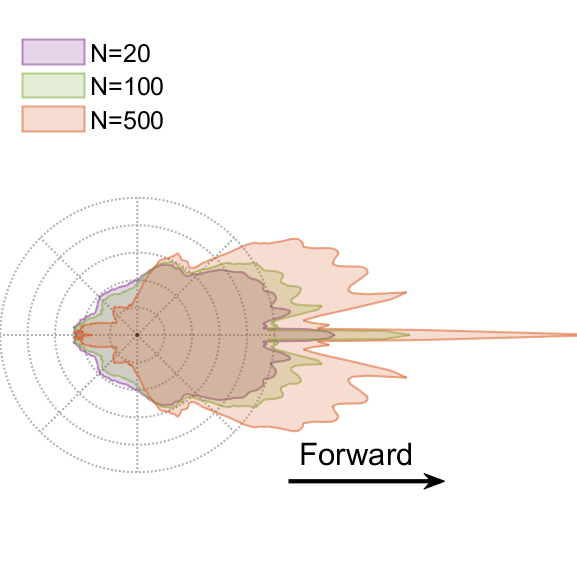
\includegraphics[width=\resLen]{images/pfunc/number.png} &
        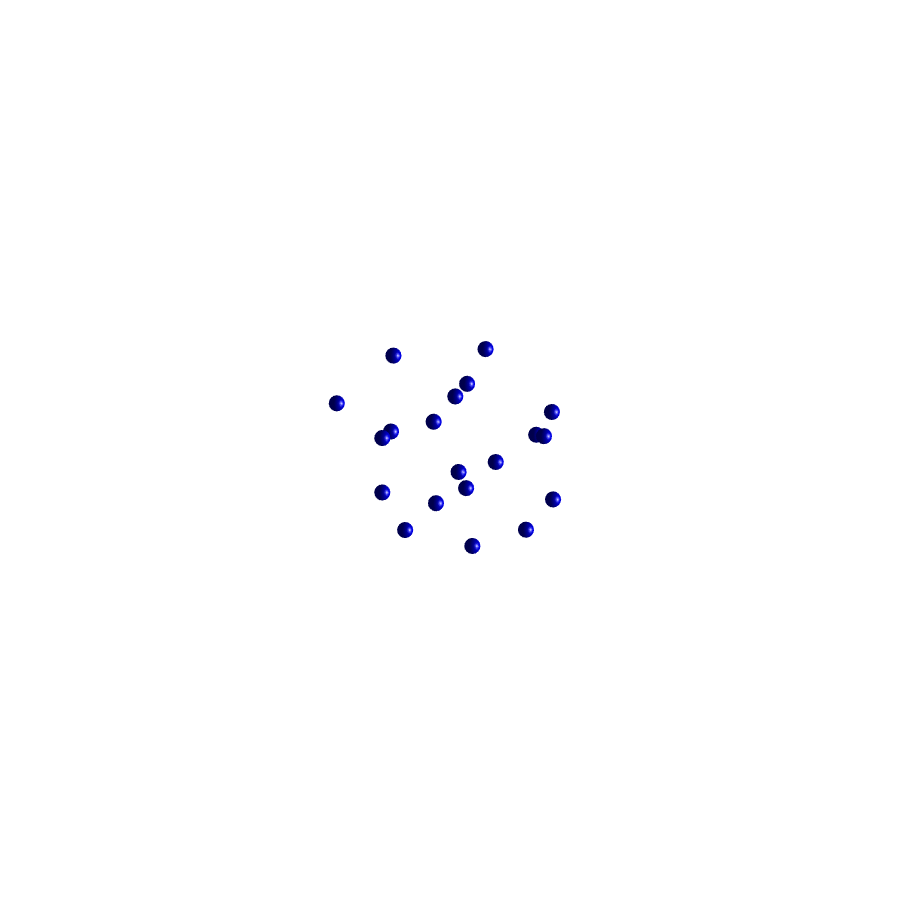
\includegraphics[width=\resLen]{images/particle/validate8_D2_N20_500nm.png} &
        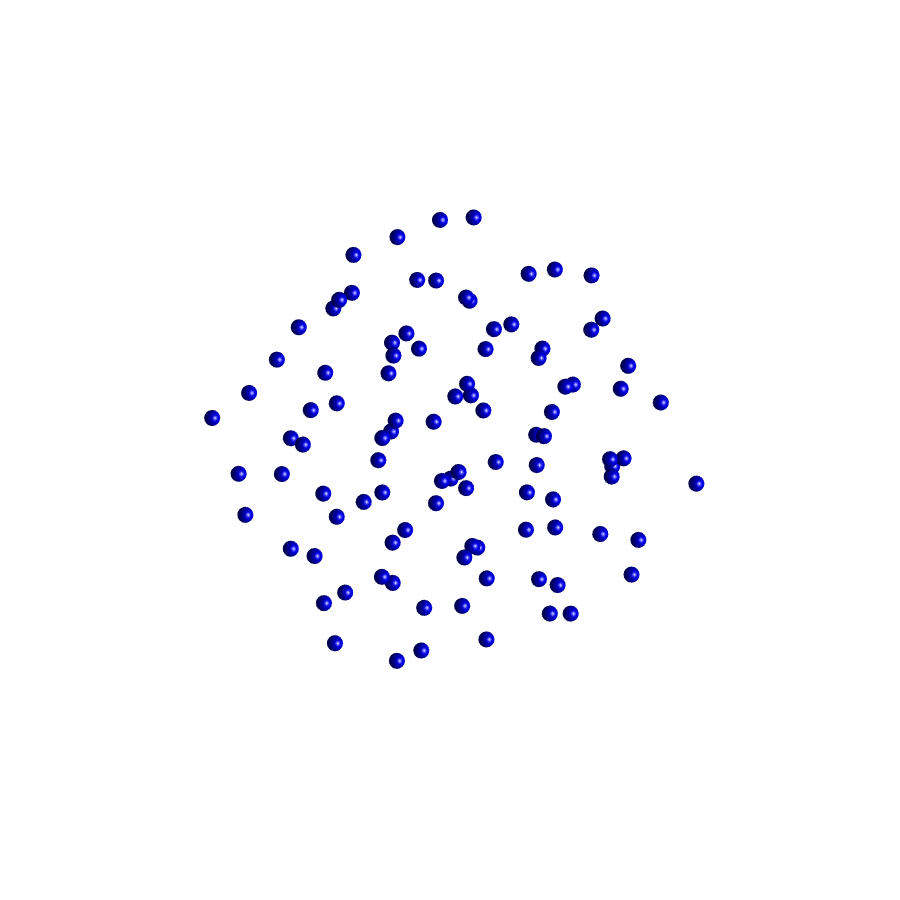
\includegraphics[width=\resLen]{images/particle/validate3_D2_N100_500nm.png} &
        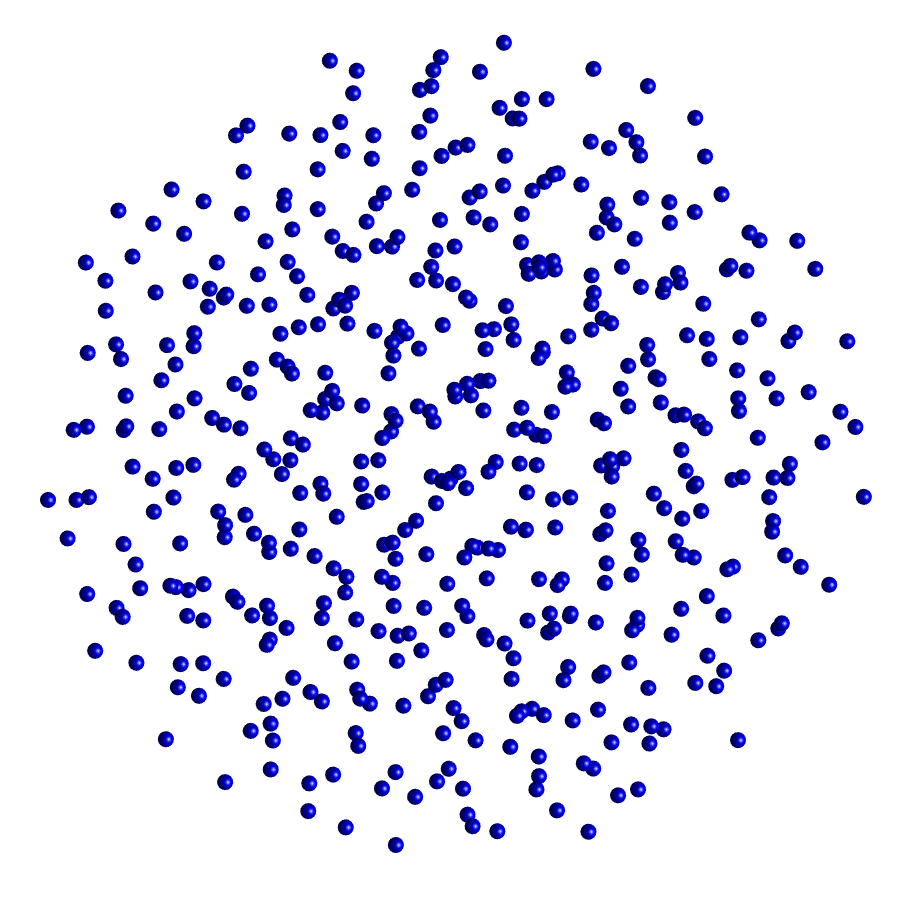
\includegraphics[width=\resLen]{images/particle/validate10_D2_N500_500nm.png} 
        \\
        Phase function & N=20 & N=100 & N=500
    \end{tabular}
    \caption{\label{fig:cluster}
        Different numbers of particle in cluster. Wavelength is 700nm, particle size is 500nm.s
    }
\end{figure}

